%-------------------------------------------------------------------------------
%	PACKAGES AND OTHER DOCUMENT CONFIGURATIONS
%-------------------------------------------------------------------------------


\documentclass[a4paper,12pt]{article}
\usepackage[english]{babel}
% \usepackage[latin1]{inputenc}
\usepackage{amsmath}
\usepackage{amssymb}
\usepackage{amsfonts}
\usepackage{graphicx}
\usepackage{dcolumn}
\usepackage[colorinlistoftodos]{todonotes}
\usepackage[toc,page]{appendix}
\usepackage{setspace}
% \doublespacing
\usepackage{tcolorbox}
\tcbuselibrary{skins}
\usepackage{booktabs}
\usepackage{hyperref}
\usepackage{geometry}
\usepackage[bottom]{footmisc}
\usepackage{listings}
\usepackage{longtable}
% \usepackage[demo]{graphicx}
\usepackage{subfig}
\usepackage{multirow}
\usepackage{tikz}
\usetikzlibrary{fit}
\usetikzlibrary{arrows}
\renewcommand{\arraystretch}{0.7}
\renewcommand{\labelitemi}{$\triangleright$}
 \geometry{
 a4paper,
 total={170mm,257mm},
 left=25mm,
 top=30mm,
 right=25mm,
 bottom=25mm,
 }
 \usepackage{hyperref}
 \hypersetup{
    bookmarks=true,         % show bookmarks bar?
    unicode=false,          % non-Latin characters in Acrobat’s bookmarks
    pdftoolbar=true,        % show Acrobat’s toolbar?
    pdfmenubar=true,        % show Acrobat’s menu?
    pdffitwindow=false,     % window fit to page when opened
    pdfstartview={FitH},    % fits the width of the page to the window
    pdftitle={Design_Report},    % title
    pdfauthor={Jacob Pichelman, Luca Poll},     % author
    pdfsubject={Subject},   % subject of the document
    pdfcreator={Creator},   % creator of the document
    pdfproducer={Producer}, % producer of the document
    pdfkeywords={keyword1, key2, key3}, % list of keywords
    pdfnewwindow=true,      % links in new PDF window
    colorlinks=false,       % false: boxed links; true: colored links
    linkcolor=red,          % color of internal links (change box color with linkbordercolor)
    citecolor=green,        % color of links to bibliography
    filecolor=magenta,      % color of file links
    urlcolor=cyan           % color of external links
}

\definecolor{Gray}{gray}{0.9}
% \setmonofont{Consolas}

\definecolor{background}{RGB}{39, 40, 34}
\definecolor{string}{RGB}{230, 219, 116}
\definecolor{comment}{RGB}{117, 113, 94}
\definecolor{normal}{RGB}{248, 248, 242}
\definecolor{identifier}{RGB}{166, 226, 46}

\lstset{
  language = R,                         % choose the language of the code
  linewidth = 14.75cm,
  numbers = left,                           % where to put the line-numbers
  stepnumber=1,                         % the step between two line-numbers.        
  numbersep=5pt,                        % how far the line-numbers are from the code
  numberstyle=\tiny\color{black}\ttfamily,
  backgroundcolor=\color{background},       % choose the background color. You must add \usepackage{color}
  showspaces=false,                     % show spaces adding particular underscores
  showstringspaces=false,               % underline spaces within strings
  showtabs=false,                       % show tabs within strings adding particular underscores
  tabsize=4,                            % sets default tabsize to 2 spaces
  captionpos=b,                         % sets the caption-position to bottom
  breaklines=true,                      % sets automatic line breaking
  breakatwhitespace=true,               % sets if automatic breaks should only happen at whitespace
  title=\lstname,                       % show the filename of files included with \lstinputlisting;
  basicstyle=\color{normal}\ttfamily,                   % sets font style for the code
  keywordstyle=\color{magenta}\ttfamily,    % sets color for keywords
  stringstyle=\color{string}\ttfamily,      % sets color for strings
  commentstyle=\color{comment}\ttfamily,    % sets color for comments
  emph={format_string, eff_ana_bf, permute, eff_ana_btr},
  emphstyle=\color{identifier}\ttfamily
}

% biblatex
\usepackage{biblatex}
\addbibresource{references.bib}
\usepackage{csquotes}


\begin{document}
\begin{titlepage}

\newcommand{\HRule}{\rule{\linewidth}{0.25mm}} % Defines a new command for the horizontal lines, change thickness here
\setlength{\topmargin}{-0.5in}
\center % Center everything on the page


\includegraphics[scale=0.75]{TSE.png}\\

%-------------------------------------------------------------------------------
%	HEADING SECTIONS
%-------------------------------------------------------------------------------
% \\[1.5cm]
\large \textsc{M2 EEE Machine Learning} 
\vspace{1.5cm}
% Name of your heading such as course name
\textsc{\large } % Minor heading such as course title

%-------------------------------------------------------------------------------
%	TITLE SECTION
%-------------------------------------------------------------------------------

\HRule \\[0.75cm]
{ \huge \bfseries Final Project}\\[0.5cm] % Title of your document
\HRule \\[1.75cm]
 
%-------------------------------------------------------------------------------
%	AUTHOR SECTION
%-------------------------------------------------------------------------------

\large\textsc{Andrew Boomer and Jacob Pichelmann} \\[1.5cm]

%-------------------------------------------------------------------------------
%	DATE SECTION
%-------------------------------------------------------------------------------

{\large \today}\\[0.5cm] % Date, change the \today to a set date if you want to be precise

\vfill % Fill the rest of the page with whitespace

\end{titlepage}

% -------------------------------------------------------------
% TABLE OF CONTENTS
\renewcommand{\contentsname}{Table of Contents}
\tableofcontents
% -------------------------------------------------------------

\newpage

\section{Introduction}

Four dimension reduction devices: (1) Principal Component Analysis, (2) Ridge Regression, (3) Landweber Fridman (LF) regularization, (4) Partial least squares. Each involves a regularization or tuning parameter that is selected through genearlized cross validation (GCV). 

Take two different data generating processes, (1) The eigenvalues of $\frac{X^{'}X}{T}$ are bounded and decline to zero gradually. (2) Popular factor model with a finite number, r, of factors. Here, the r largest eigenvalues grow with N, while the remaining are bounded. In both cases, $\frac{X^{'}X}{T}$ is ill-conditioned, which means the ratio of the largest to smallest eigenvalue diverges, and a regularization terms is needed to invert the matrix.

\section{Data Generating Process}

Large Sample Case: $N = 200$ and $T = 500$
Small Sample Case: $N = 100$ and $T = 50$

\[\underbrace{x_{t}}_{(N \times 1)} = \underbrace{\Lambda}_{(N \times r)} \underbrace{F_{t}}_{(r \times 1)} + \underbrace{\xi_{t}}_{(N \times 1)}\]

\[\underbrace{y_{t}}_{(1 \times 1)} = \underbrace{\theta^{'}}_{(1 \times r)} \underbrace{F_{t}}_{(r \times 1)} + \underbrace{\nu_{t}}_{(1 \times 1)}\]

\[\underbrace{y}_{(T \times 1)} = \underbrace{F}_{(T \times r)} \underbrace{\theta}_{(r \times 1)} + \underbrace{\nu}_{(T \times 1)}\]

\[\underbrace{X}_{(T \times N)} = \underbrace{F}_{(T \times r)} \underbrace{\Lambda^{'}}_{(r \times N)} + \underbrace{\xi}_{(T \times N)}\]

DGP 1 (Few Factors Structure):
$\theta$ is the $(r \times 1)$ vector of ones, $r = 4$ and $r_{max} = r + 10$

DGP 2 (Many Factors Structure):
$\theta$ is the $(r \times 1)$ vector of ones, $r = 50$ and $r_{max} = min(N, \frac{T}{2})$

DGP 3 (Five Factors but only One Relevant):
$\theta = (1, 0_{1 \times 4})$, $r = 5$ and $r_{max} = min(r + 10, min(N, \frac{T}{2}))$

$F = [F_{1}, F_{2}^{'}]^{'}$ and $F \times F^{'} = \begin{bmatrix} 1 & 0 & 0 & 0 & 0 \\ 0 & 2 & 0 & 0 & 0 \\ 0 & 0 & 3 & 0 & 0 \\ 0 & 0 & 0 & 3 & 0 \\ 0 & 0 & 0 & 0 & 4\end{bmatrix}$

$y = \hat{F} \theta + \nu$ where $\hat{F}$ is generated from $X$ equation in DGP 3, and $\sigma_{\nu} = 0.1$

DGP 4 ($x_{t}$ Has a Factor Structure but Unrelated to $y_{t}$):

$\theta$ is a vector of zeros with dimension $(r \times 1)$. $r = 5$, $r_{max} = r + 10$. $F \times F^{'}$ is defined as in DGP 3.

DGP 5 (Eigenvalues Declining Slowly):

$\theta$ is an $(N \times 1)$ vector of ones. $r = N$, $r_{max} = min(N, \frac{T}{2}$.

$\Lambda = M \odot \xi$, with $\xi \sim (N \times N)$ matrix of $iidN(0, 1)$

$M \sim (N \times N) = \begin{bmatrix} 1 & 1 & \dotsb & 1 \\ \frac{1}{2} & \frac{1}{2} & \dotsb & \frac{1}{2} \\ \vdots & \vdots & \vdots & \vdots \\ \frac{1}{N} & \frac{1}{N} & \dotsb & \frac{1}{N}\end{bmatrix}$

DGP 6 (Near Factor Model):

$\theta = 1$, $r = 1$, $r_{max} = r + 10$, $\Lambda^{'} = \frac{1}{\sqrt{N}}1_{r \times N}$


Estimation:

Set 1: Bai-Ng, PCA, PLS, Ridge, LF, LASSO
Set 2: GCV, Mallows, AIC, BIC
Set 3: Small Sample, Large Sample

Parameter Iteration (For Later)
Simulation (Andy)
Model Estimation (Jacob)
Evaluation (Jacob)
Output (Andy)

\section{Estimation Methods}

Ridge Estimator:

\[\widehat{y} = M_{T}^{\alpha} y = X (S_{xx} + \alpha I)^{-1} S_{xy}\]

LF Estimator:

\[\widehat{y} = M_{T}^{\alpha} y = X \sum_{j=1}^{\min (N, T)} \frac{\left(1-\left(1-d \widehat{\lambda}_{j}^{2}\right)^{1 / \alpha}\right)}{\widehat{\lambda}_{j}^{2}}\left\langle y, \hat{\psi}_{j}\right\rangle_{T} \frac{X^{\prime} \hat{\psi}_{j}}{T}\]

Spectral Cutoff/Principal Components Estimator:

\[\widehat{y} = M_{T}^{\alpha} y = \widehat{\Psi} \left(\widehat{\Psi}^{\prime} \widehat{\Psi}\right)^{-1} \widehat{\Psi}^{\prime} y\]

\[\text{ Where } \widehat{\Psi} = \left[\widehat{\psi}_{1}\left|\widehat{\psi}_{2}\right| \ldots \mid \widehat{\psi}_{k}\right]\]

Partial Least Squares Estimator:

\[\widehat{y} = M_{T}^{\alpha} y = X V_{k}\left(V_{k}^{\prime} X^{\prime} X V_{k}\right)^{-1} V_{k}^{\prime} X^{\prime} y\]

\[\text{ Where } V_{k}=\left(X^{\prime} y, \quad\left(X^{\prime} X\right) X^{\prime} y, \ldots,\left(X^{\prime} X\right)^{k-1} X^{\prime} y\right)\]

\subsection{Via SIMPLS Algorithm}

\begin{align}
\nonumber S = X^{T} y & \\
\nonumber \text{for } & i \in 1:k \\
\nonumber &\text{if } i = 1, [u, s, v] = svd(S) \\
\nonumber &\text{if } i > 1, [u, s, v] = svd(S - (P_{k}[:, i-1](P_{k}[:, i-1]^{T} P_{k}[:, i-1])^{-1} P_{k}[:, i-1]^{T} S)) \\
\nonumber &T_{k}[:, i - 1] = X R_{k}[:, i - 1] \\
\nonumber &P_{k}[:, i - 1] = \frac{X^{T} T_{k}[:, i - 1]}{T_{k}[:, i - 1]^{T}T_{k}[:, i - 1]} \\
\nonumber \widehat{y} = M^{\alpha}_{T} y &= X R_{k} (T^{T}_{k} T_{k})^{-1} T^{T}_{k} y
\end{align}

\section{Evaluation Methods}

Generalized Cross Validation:

\[\hat{\alpha}=\arg \min _{\alpha \in A_{T}} \frac{T^{-1}\left\|y-M_{T}^{\alpha} y\right\|^{2}}{\left(1-T^{-1} \operatorname{tr}\left(M_{T}^{\alpha}\right)\right)^{2}}\]

Mallows Criterion:

\[\hat{\alpha}=\arg \min _{\alpha \in A_{T}} T^{-1}\left\|y-M_{T}^{\alpha} y\right\|^{2}+2 \widehat{\sigma}_{\varepsilon}^{2} T^{-1} \operatorname{tr}\left(M_{T}^{\alpha}\right)\]

\[\text{ Where } \widehat{\sigma}_{\epsilon}^{2} \text{ is a consistent estimator of the variance of } \epsilon\]

So variance of $\epsilon$ is taken from the errors of the largest model, or from the model with all regressors for PC.

Leave-one-out Cross Validation:

\[\hat{\alpha}=\arg \min _{\alpha \in A_{T}} \frac{1}{T} \sum_{t=1}^{T}\left(\frac{y_{i}-\hat{y}_{i, \alpha}}{1-M_{T}^{\alpha}[ii]}\right)^{2}\]

\input{Table_N100_T50_EvalGCV_Sims50}

\clearpage

\section{Empirical Application}
\subsection{Introduction and Data}
Building on the long history of machine learning in forecasting macroeconomic variables\footnote{See e.g. ...} we use the Federal Reserve Bank's monthly database (FRED-MD) to apply the estimators discussed above on real data. This database was established for empirical analysis that requires 'big data' and hence constitutes an ideal environment to employ the methods discussed above. We took inspiration from the work of Coulombe et al. (2020) but limit ourselves to PC, Ridge, PLS and LF.\footnote{Unfortunately we were unable to use (1) Gu et al. (2020) as TSE does not have access to WDRS returns, (2) as only data on the resulting factors is available or (3) as they do not offer any replication data.} 
The dataset contains 134 monthly US macroeconomic and financial indicators observed from January 1959 to January 2021. An overview of all variables is given in the appendix. 
Following Coulombe et al. (2020) we predict three indicators which are of key economic interest, namely Industrial Production (INDPRO), Unemployment Rate (UNRATE), and the Consumer Price Index (INF).\footnote{Fortunately McCracken and Ng (2016), the accompanying paper of the dataset, outlines a transformation method for each variable to achieve stationarity. We apply those transformations in our data preparation.}
For each of these variables of interest $Y_t$ we follow Coulombe et al (2020) in defining the forecast objective as

\begin{align}
	y_{t+h} = (1/h) ln(Y_{t+h}/Y_t)
\end{align}

where $h$ denotes the number of periods ahead. This allows us to assess the performance of our predictive methods for further periods ahead.

\subsection{Evaluation}
We evaluate the performance of our methods on two metrics, in-sample MSE and out of sample MSE. To be able to compute the latter we split our data into a training and a test set where the former spans all observations from ... to ... amounting to 80\% of the data. We conduct forecasts for $h = \{1, 3, 9\}$ periods ahead. In line with the findings of Coulombe et al (2020) we observe that the performance increases for further periods ahead. Given the simulation results we expect Ridge to deliver the best results, here defined as yielding the smallest MSE, both in sample and out of sample. Importantly we find that the number of factors $k$ as well as the penalty parameter $\alpha$ are very stable across all methods of parameter tuning (i.e. GCV, Mallows, LOO-CV) and across dependent variables. We were unable to discover evidence supporting nor disputing this finding in the literature related to the usage of FRED-MD.\footnote{We apply the same exact estimators as in the simulations hence we see room for error only in our data preparation steps, which are, however, directly taken from the literature. Given the nature of the data we might take this finding as an indication for a stable factor structure. Future research could discover interesting patterns.} We therefore only report the tuning parameters in the appendix. 

\subsection{Results and Discussion}
Given the similarity of the selected tuning parameters we only show MSE estimates for parameters selected by GCV.\footnote{For details see table \ref{}}

\begin{tabular}{lllrrrr}
\toprule
{} &  Target &         Method &    MSE\_is &   MSE\_oos &    opt\_par &  horizon \\
\midrule
22 &   HOUST &        LF: GCV &  0.005382 &  0.007627 &   0.000117 &        1 \\
23 &   HOUST &     LF: Mallow &  0.005382 &  0.007627 &   0.000117 &        1 \\
4  &   HOUST &        PC: GCV &  0.005383 &  0.010409 &  15.000000 &        1 \\
5  &   HOUST &     PC: Mallow &  0.005383 &  0.010409 &  15.000000 &        1 \\
16 &   HOUST &       PLS: GCV &  0.005748 &  0.329750 &  11.000000 &        1 \\
17 &   HOUST &    PLS: Mallow &  0.005748 &  0.238590 &  15.000000 &        1 \\
10 &   HOUST &     Ridge: GCV &  0.005016 &  0.008906 &   0.117000 &        1 \\
11 &   HOUST &  Ridge: Mallow &  0.005016 &  0.008906 &   0.117000 &        1 \\
18 &  INDPRO &        LF: GCV &  0.000051 &  0.000126 &   0.000117 &        1 \\
19 &  INDPRO &     LF: Mallow &  0.000051 &  0.000126 &   0.000117 &        1 \\
0  &  INDPRO &        PC: GCV &  0.000053 &  0.000162 &  13.000000 &        1 \\
1  &  INDPRO &     PC: Mallow &  0.000053 &  0.000162 &  15.000000 &        1 \\
12 &  INDPRO &       PLS: GCV &  0.000055 &  0.002139 &  15.000000 &        1 \\
13 &  INDPRO &    PLS: Mallow &  0.000055 &  0.002139 &  15.000000 &        1 \\
6  &  INDPRO &     Ridge: GCV &  0.000049 &  0.000130 &   0.117000 &        1 \\
7  &  INDPRO &  Ridge: Mallow &  0.000049 &  0.000130 &   0.117000 &        1 \\
20 &  UNRATE &        LF: GCV &  0.000707 &  0.001488 &   0.000117 &        1 \\
21 &  UNRATE &     LF: Mallow &  0.000707 &  0.001488 &   0.000117 &        1 \\
2  &  UNRATE &        PC: GCV &  0.000729 &  0.002247 &   9.000000 &        1 \\
3  &  UNRATE &     PC: Mallow &  0.000729 &  0.002276 &  15.000000 &        1 \\
14 &  UNRATE &       PLS: GCV &  0.000733 &  0.031782 &  13.000000 &        1 \\
15 &  UNRATE &    PLS: Mallow &  0.000733 &  0.063822 &  15.000000 &        1 \\
8  &  UNRATE &     Ridge: GCV &  0.000677 &  0.001779 &   0.117000 &        1 \\
9  &  UNRATE &  Ridge: Mallow &  0.000677 &  0.001779 &   0.117000 &        1 \\
\bottomrule
\end{tabular}


%\newcolumntype{M}[1]{>{\centering\arraybackslash}m{#1}}
\begin{table}[]
    \centering
    \begin{tabular}{c}
        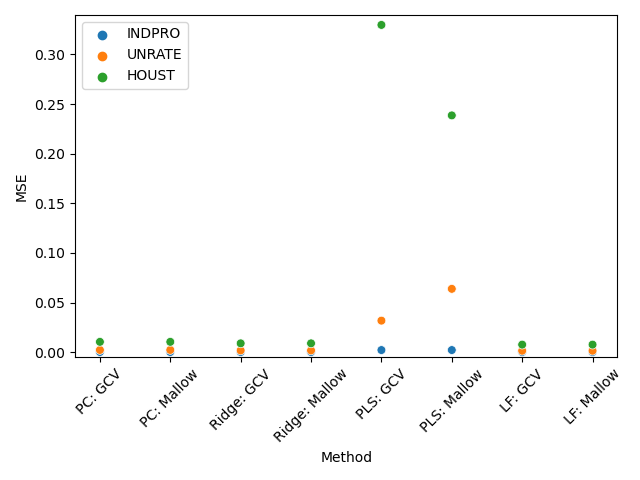
\includegraphics[width=0.6\textwidth]{figures/MSE_oos_h1.png} \\
        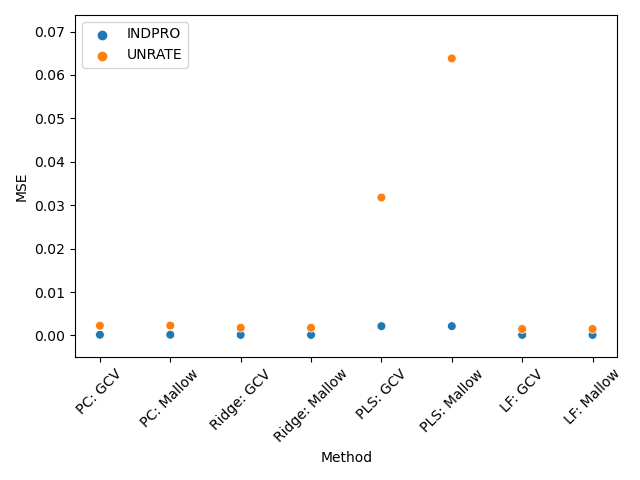
\includegraphics[width=0.6\textwidth]{figures/MSE_oos_h1_noHOUST.png}
    \end{tabular}
    \caption*{Out of sample MSE, $h = 1$}
\end{table}

\begin{table}[]
    \centering
    \begin{tabular}{c}
        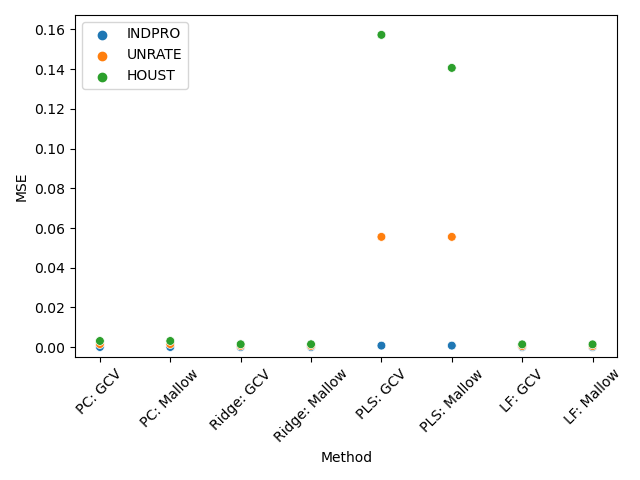
\includegraphics[width=0.6\textwidth]{figures/MSE_oos_h3.png} \\
        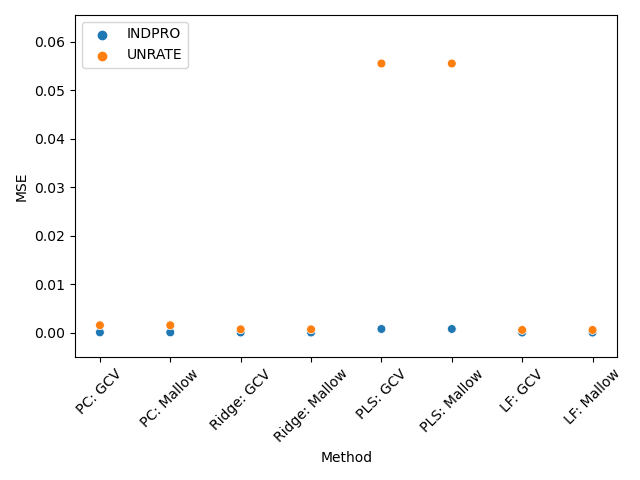
\includegraphics[width=0.6\textwidth]{figures/MSE_oos_h3_noHOUST.png}
    \end{tabular}
    \caption*{Out of sample MSE, $h = 3$}
\end{table}

\begin{table}[]
    \centering
    \begin{tabular}{c}
        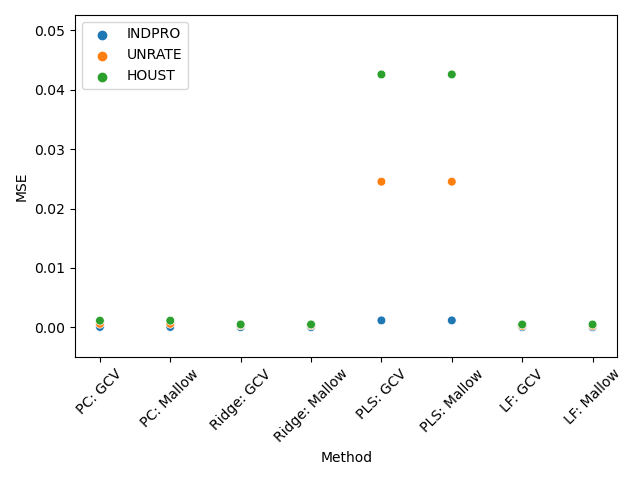
\includegraphics[width=0.6\textwidth]{figures/MSE_oos_h9.png} \\
        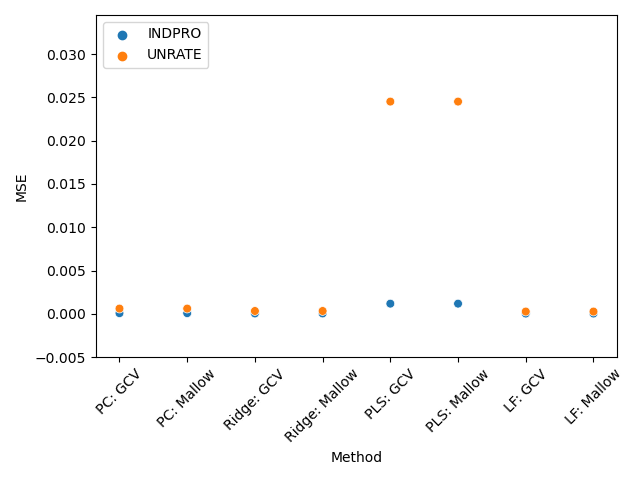
\includegraphics[width=0.6\textwidth]{figures/MSE_oos_h9_noHOUST.png}
    \end{tabular}
    \caption*{Out of sample MSE, $h = 9$}
\end{table}


\clearpage 
\section*{Appendix}

\subsection*{Data Dictionary}
\begin{figure}[h!]
        \centering
        \caption*{Group 1: Output and income}
        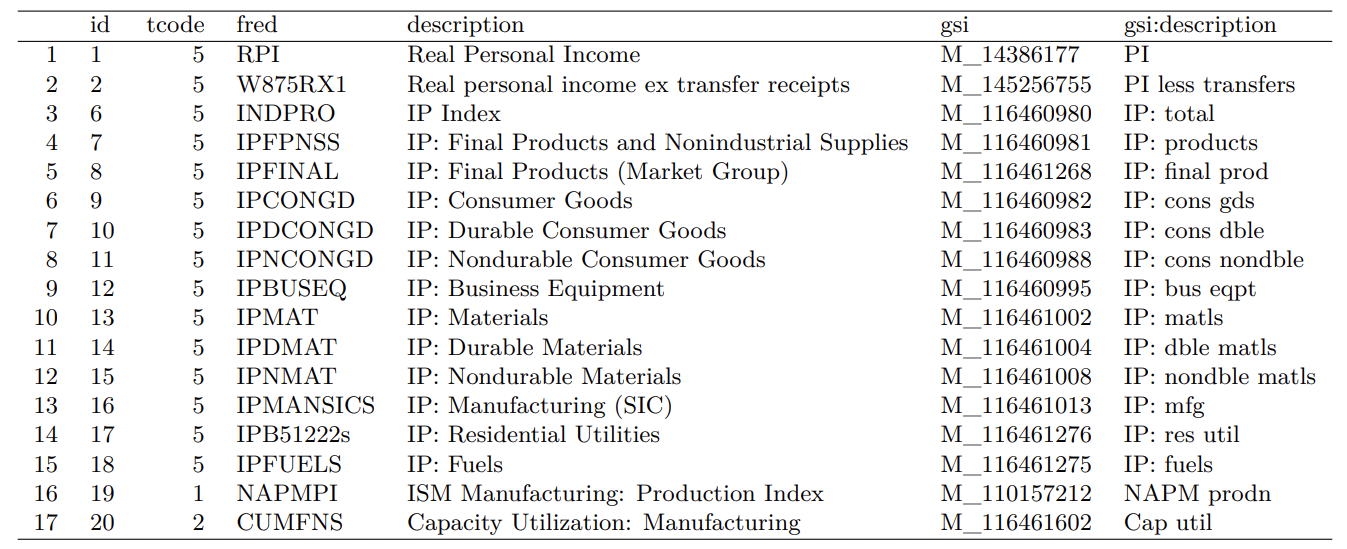
\includegraphics[width=0.9\textwidth]{figures/G1.png}
\end{figure}

\begin{figure}
        \centering
        \caption*{Group 2: Labour market}
        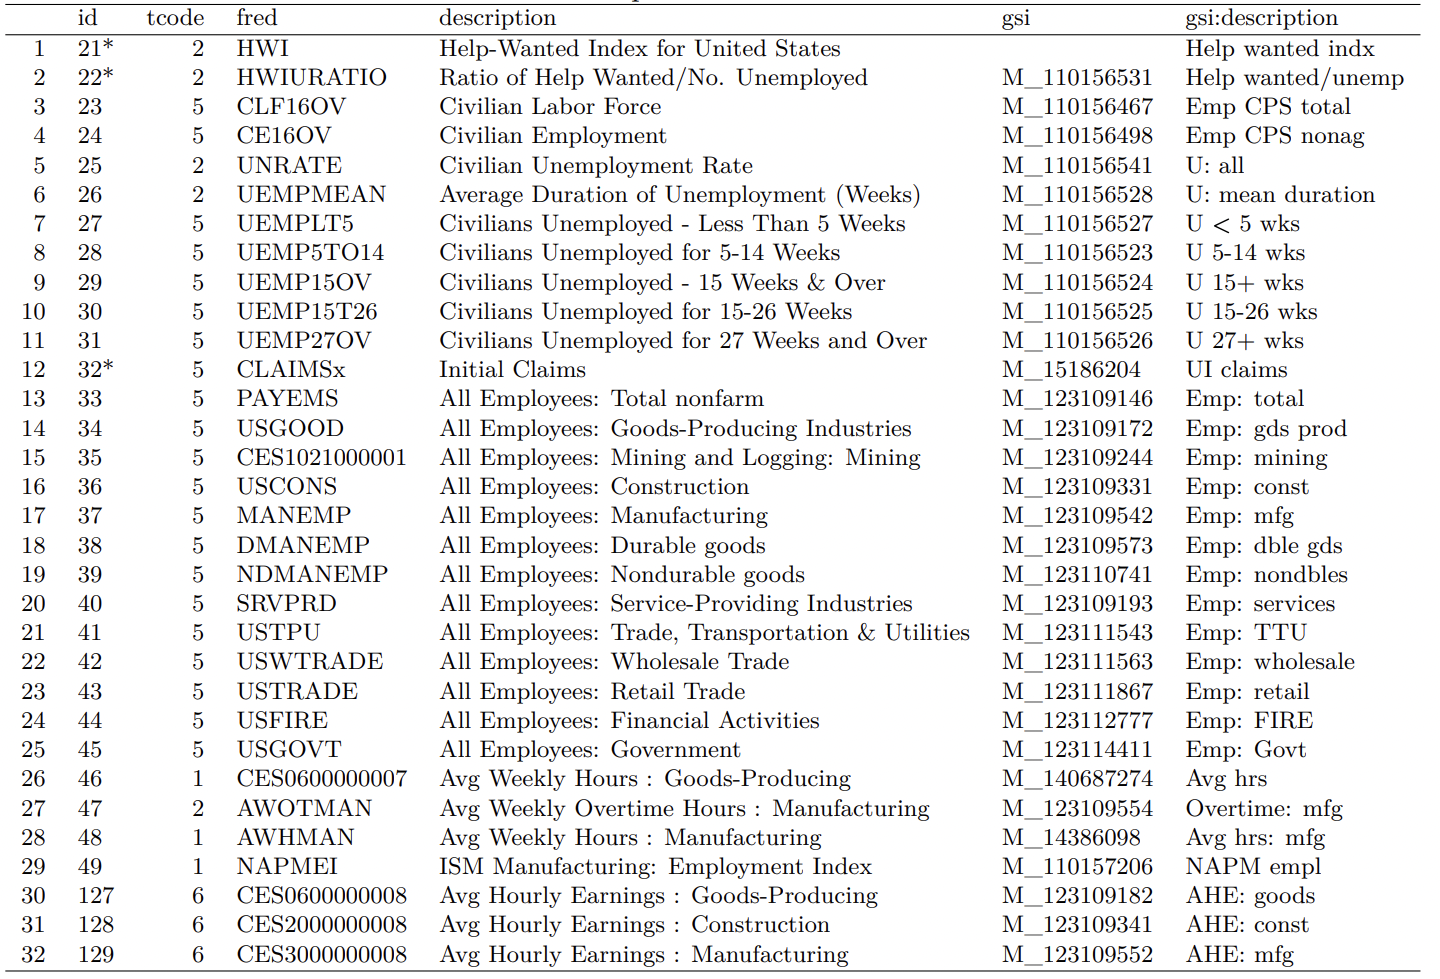
\includegraphics[width=0.9\textwidth]{figures/G2.png}
\end{figure}

\begin{figure}
        \centering
        \caption*{Group 3: Housing}
        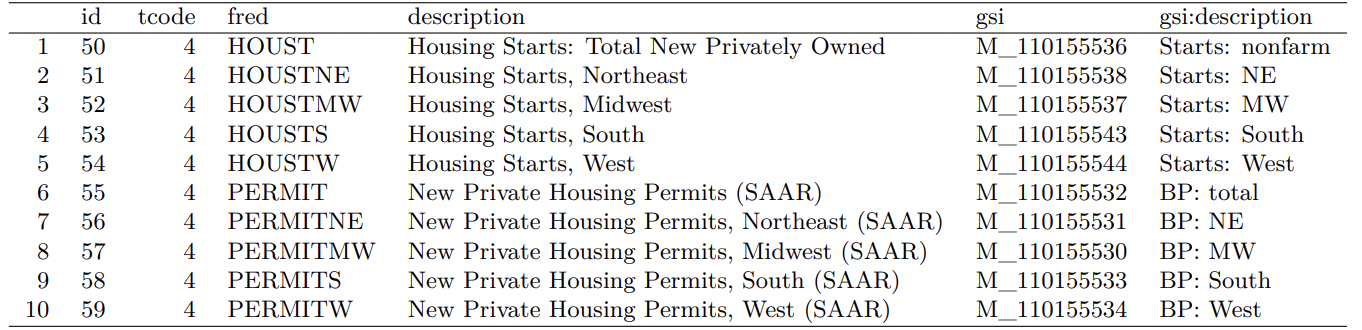
\includegraphics[width=0.9\textwidth]{figures/G3.png}
\end{figure}

\begin{figure}
        \centering
        \caption*{Group 4: Consumption, orders and inventories}
        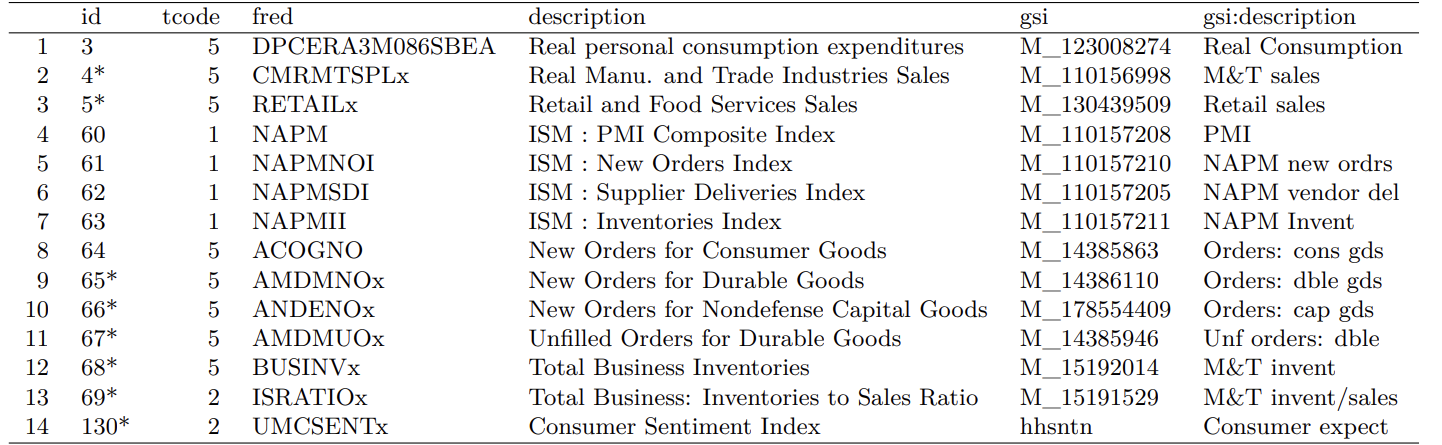
\includegraphics[width=0.9\textwidth]{figures/G4.png}
\end{figure}

\begin{figure}
        \centering
        \caption*{Group 5: Money and credit}
        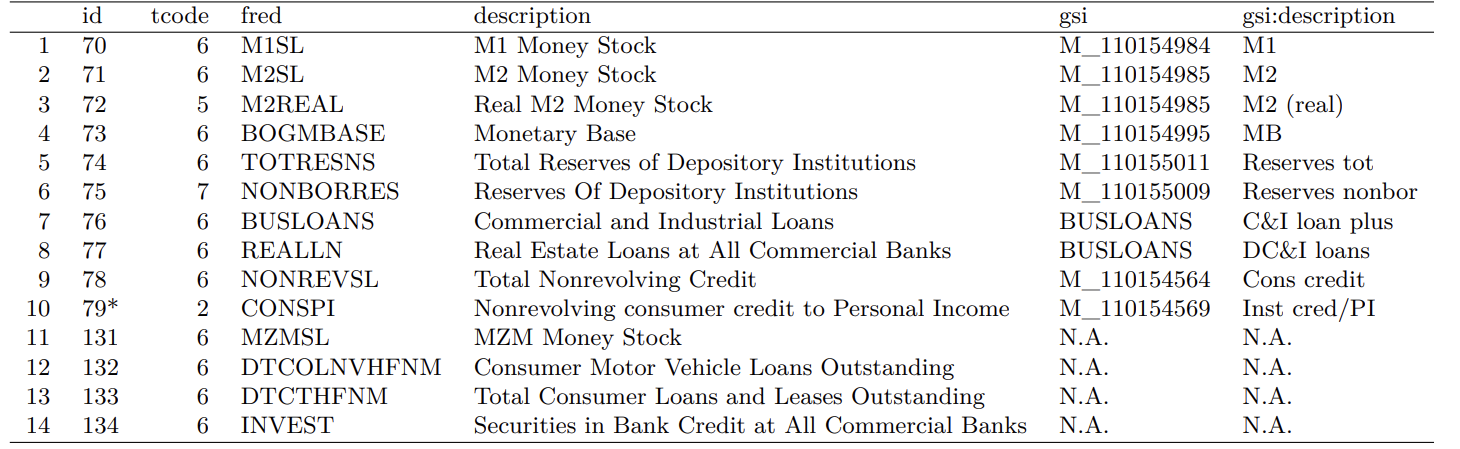
\includegraphics[width=0.9\textwidth]{figures/G5.png}
\end{figure}

\begin{figure}
        \centering
        \caption*{Group 6: Interest and exchange rates}
        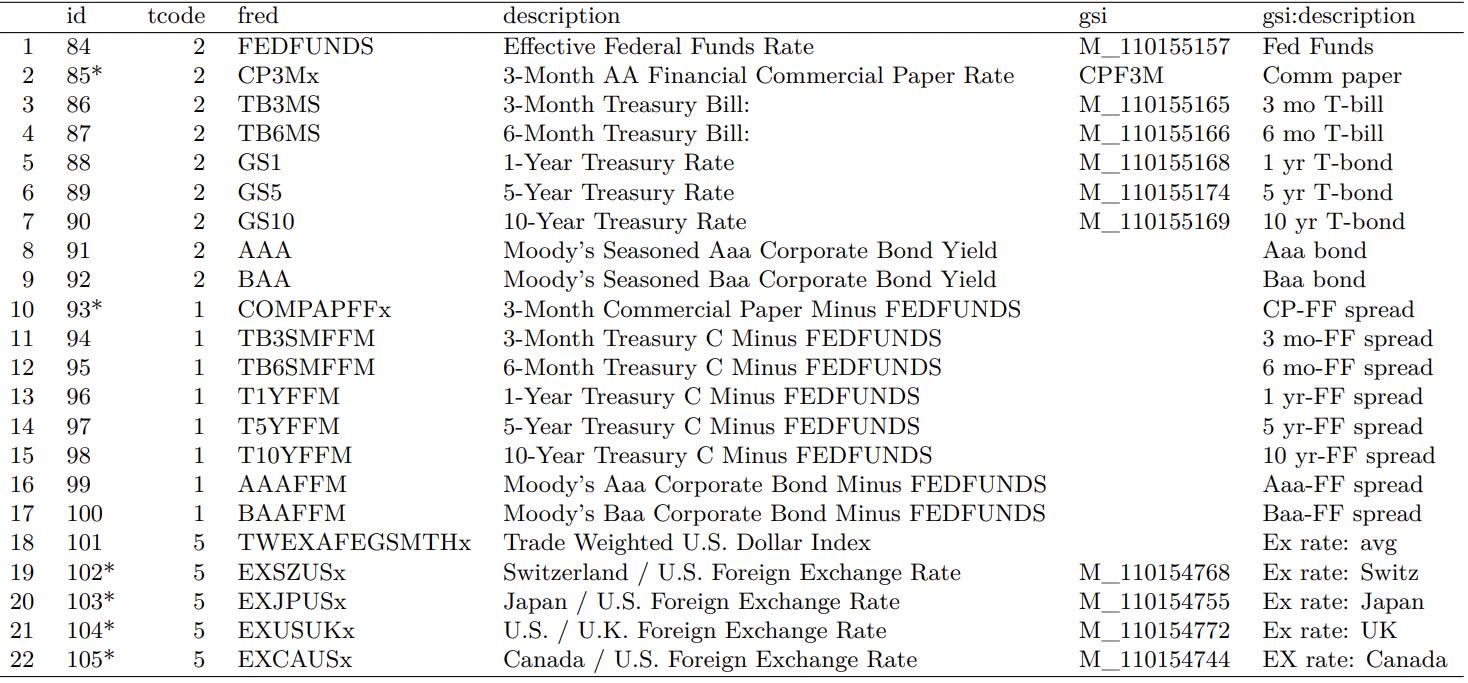
\includegraphics[width=0.9\textwidth]{figures/G6.png}
\end{figure}

\begin{figure}
        \centering
        \caption*{Group 7: Prices}
        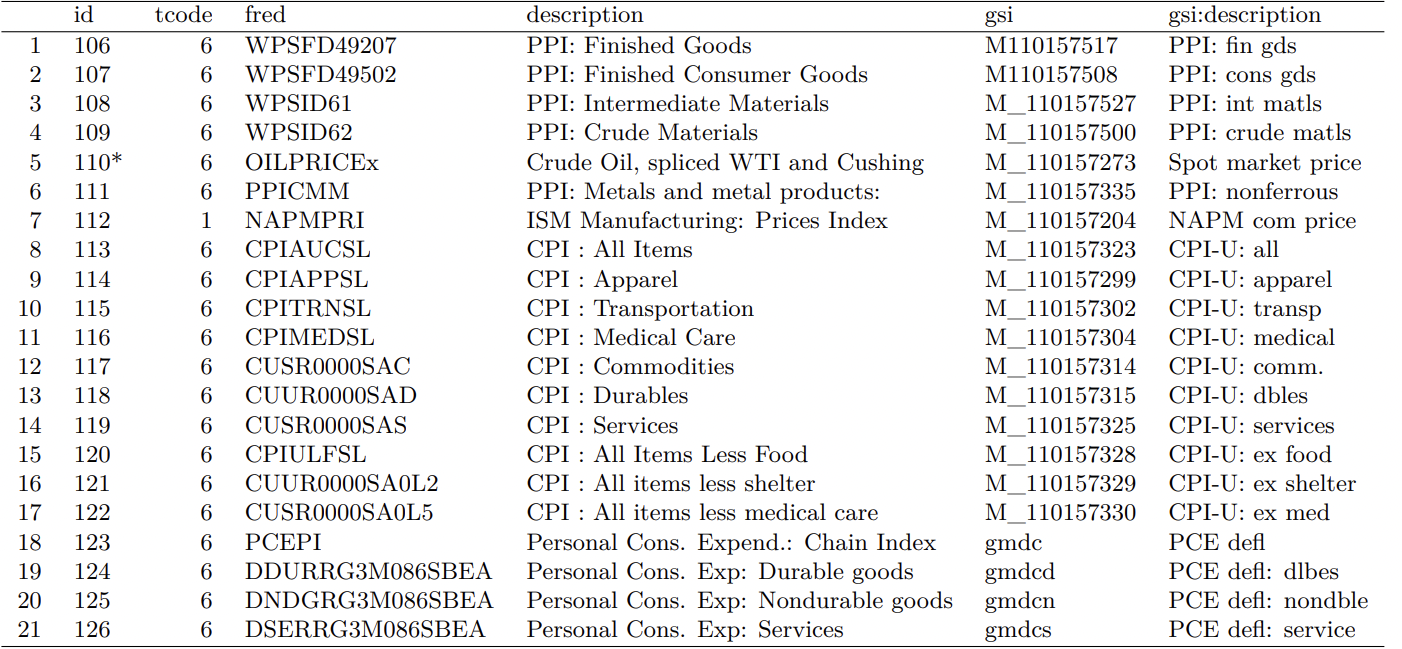
\includegraphics[width=0.9\textwidth]{figures/G7.png}
\end{figure}

\begin{figure}
        \centering
        \caption*{Group 8: Stock market}
        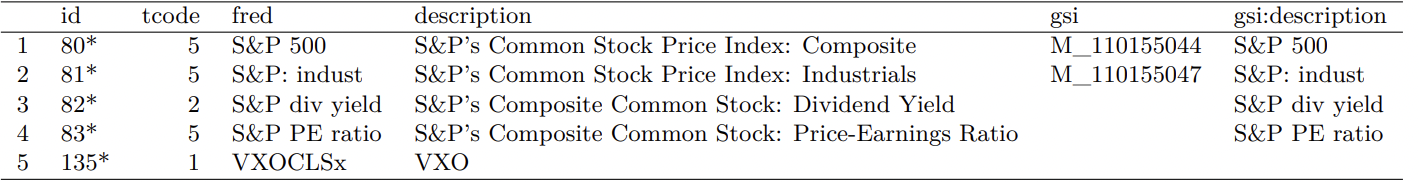
\includegraphics[width=0.9\textwidth]{figures/G8.png}
\end{figure}








\end{document}




